\documentclass[a4paper]{article}
\usepackage{INTERSPEECH2016}
\usepackage{graphicx}
\usepackage{dblfloatfix}
\usepackage[superscript,biblabel]{cite}
\usepackage{multirow,tabularx}
\usepackage{hhline}
\newcommand\independent{\protect\mathpalette{\protect\independenT}{\perp}}
\def\independenT#1#2{\mathrel{\rlap{$#1#2$}\mkern2mu{#1#2}}}
\title{Establishing Causality in Microbiome/Disease Interactions\\A
  Study in Crohn's Disease}
%\subtitle{A Study in Crohn's Disease}
\name{Daniel Speyer}
\address{dls2192@columbia.edu}
\begin{document}
\ninept

%\twocolumn[
%  \begin{@twocolumnfalse}
    \maketitle
%  \end{@twocolumnfalse}
%]

\begin{abstract}
The literature abounds with correlational studies matching diseases to
gut microbiome dysbiosis, but medical practice does not abound with
corresponding probiotic therapies.  One critical missing piece is
causality.  If the dysbiosis is a \textit{result} of the disease,
then there is no point in correcting the dysbiosis.  In this paper we
present three statistical techniques for determining causality from
existing data and apply them to Crohn's Disease.  The first technique
is to find bacteria which are the mechanism by which a gene causes the
disease.  The second is to find bacteria that correlate to the
disease, but not to that gene.  The final technique is to look for a
specific three-species motif, with a distinctive set of conditional
dependences and independences.
\end{abstract}

\begin{figure*}[t]
  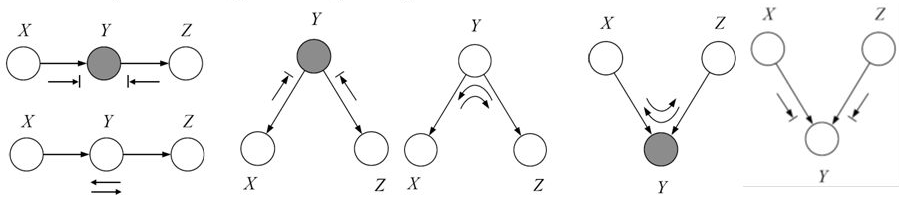
\includegraphics[width=\textwidth]{bayesball}
  \caption{The ``Bayes Ball'' rule: how mutual information travels and
  does not travel through a causal graph, as illustrated by Pan and
  Xu\cite{bayesball} }
\end{figure*}

\section{Introduction}

A great many diseases correlate with disruptions in the gut microbiome
(known as “dysbiosis”).  In addition to Crohn's Disease, these include
Metabolic Syndrome, Diabetes (both types)\cite{obesity} , Asthma, Multiple
Sclerosis\cite{autoim}, Depression and Autism\cite{cns}.  All of these diseases are
increasing in prevalence, have no clearly established cause, and are
difficult to cure.


If we knew that the disruption to the microbiome caused these
diseases, we might be able to treat or prevent them by restoring a
healthy microbiome, using probiotics or highly selective antibiotics.
Unfortunately, we only know correlation.  It is entirely possible that
the diseases cause the disruptions, or that they are both caused by
some hidden factor.  Furthermore, a healthy microbiome contains
hundreds of different species of bacteria.  Any of them might be
causes, effects or otherwise.


The gold standard for establishing causality remains the randomized
controlled trial.  While RCTs have found some success in treating
obesity with probiotics\cite{rctob}, other diseases are more difficult.  For
example, a handful of attempts have been made for treating Crohn's
Disease this way.  Early studies showed some benefit, but suffered
from small sample size or dubious endpoint choices.   A pair of larger
follow-up studies failed to find significant effect.\cite{rctma}  The studies
used a variety of bacterial species, and provided very little
explanation for how the species were chosen.  Performing large RCTs
for all plausible bacterial species and cocktails is not practical.


Our goal in this paper will be to find bacteria that are likely to
cure or prevent Crohn's Disease without an RCT.  Why Crohn's Disease?
As an autoimmune disorder of the intestine, it is particularly likely
to be caused by gut dysbiosis.  Also, while it is neither as common as
obesity nor as severe as Multiple Sclerosis, it does affect roughly
one in five hundred Americans, have a death rate 0.6 percentage points
higher than demographically matched controls\cite{mort}, and have a
quality of life impact of 0.88 during remission and 0.74 during
flare\cite{qol}.  Finally, it is a well-studied disease, with plentiful data
available through NCBI.

To establish causality, we will make use of the ``Bayes ball'' rule.
Specifically, two variables will correlate if and only if you can
trace a path between them through a causal graph changing direction
only at causes that are not controlled for or at effects which are,
and passing through things that are not (illustrated in figure 1).  This
principle is widely used in machine learning, specifically applying
bayesian models.  It can also be used in reverse to take correlational
data and find aspects of the underlying causal graph.\cite{causal}



\section{Methods}

First, microbiome and health data from 139 patients\cite{data} was
obtained. The microbiome data was
converted  to species names using BLAST and NCBI's
16S database.  For reads with multiple matches, the highest
scoring were taken.  Reads with no matches were simply dropped.  
The number of reads for each patient and each species were counted, and divided
by the total number of reads for that patient.  Uninteresting bacteria
were filtered out
by bucketing into powers of 10 and dropping
anything with an entropy below 0.5, on the logic that a bacterium that
didn't vary much between patients couldn't have interesting effects.

The read fractions were converted to boolean values by comparing them to
per-species thresholds.  For each species, a threshold was chosen that
maximized the number of Crohn's Disease statuses that could be
correctly predicted by that bacteria alone.  These boolean values can
then be thought of as ``has a clinically relevant dosage of the
bacterium''.

Similarly, Crohn's status was converted to a boolean by accepting only
Ileal Disease and Control, dropping all others.  I tried combining
Ileal CD and Colitis, but this produced nonsensical results.  For
NOD2, both mutant forms were merged into one category.  This produced exclusively
boolean variables, which made analysis considerably easier.

\subsection{The Intermediation Technique}

NOD2 is a gene, mutations in which are known\cite{data} to correlate with
Crohn's Disease.  It has been speculated that this effect is
intermediated by gut bacteria.  The first approach is to search for
those bacteria.

First. species that are linked to both NOD2 and ICD were sought.
Then  those species were controlling for and it was checked whether
this  made NOD2 and
ICD independent.  That should happen if and only if the species
intermediates.

In this case, using a standard dependence test (e.g. $\chi^2$) and
failing to reject independence does not suffice.  That cannot
distinguish between independence and an underpowered test, and
controlling for a variable decreases the power of a test.  

Instead, a special ``severing'' test was used.  This test uses four
``expected'' relationships between NOD2 and ICD.  In one, they are
independent.  In another, they are as they were before controlling,
except with $N$ decreased appropriately.  In the next, NOD2 values are
taken from the observation and ICD values are chosen based on those
using the pre-control conditional probabilities.  The last is the
same, but
the same the other way around.  Likelihood values are then computed for
all four models using a $\chi^2$ pdf.  For each model,  the
'bacterium present' and 'bacterium absent' cases are multiplied.  Finally, the
likelihood score for the 'independent' model are divided by the highest of the
competing scores to get a bayes factor.

\subsection{The Gene/Bacterium Technique}

\begin{figure}[t!]
  \includegraphics[width=.47\textwidth]{diagram_main1v2}
  \caption{Threshold-finding and the Gene/Bacterium technique
    illustrated for Eubacterium rectale as a set of data flows}
\end{figure}

NOD2 can also be useful for bacteria that are not linked to it.  Since
the mechanisms that control genes are well understood, it is safe to assume
that the gene causes the disease.  This can be combined with the two simplest
cases for the bacterium: that it causes the disease or is
caused by it, to get known three-node graphs with consequences for the
NOD2/bacteria relationship.  If the bacteria causes the disease, they
should be independent from
NOD2, but if the reverse, there should be a specific level of dependence.

The probabilities $p(NOD2)$, $p(ICD|NOD2)$ and
$p(bacterium|ICD)$ can be easily computed, and from these and the
model $p(bacterium|NOD2)$ can be predicted.  
The observed NOD2/bacterium relationship was then compared to each prediction
using a $\chi^2$ test.  The dataset was too small to
reject either hypothesis, but it was possible to use the pdf of the distribution
to produce an odds ratio.  Since neither hypothesis is ``null'' in the
classical sense, this is useful.  This paper shall refer to this test as a
``direction'' test, and it is illustrated in figure 2.

\subsection{The Three Bacterium Technique}

\begin{figure}
  \includegraphics[width=.47\textwidth]{motif2}
  \caption{The needed motif for the Three Bacterium Technique}
\end{figure}

A third technique does not rely on genomic data.  Instead, cases where
some common factor effected three different
bacteria, one of which effected Crohn's Disease were sought.  The first part is
straightforward: in such trios all pairs correlated
and continued to do so after controlling for each of the others.  A
common cause is the only simply-connected structure that produces that
effect.  The sign of the disease link is that  one bacterium in the
trio to severed
another from the disease (using the same severing test as in the
Intermediation technique).  This paper shall refer to the bacterium that does the
severing as the ``bacterium of interest'', the severed as the ``helper
bacterium'' and the third as the ``trio-maker''.  The
bacterium of interest must causes the disease, because if it were caused by
it or had a mutual cause, it would not produce a link between the
disease and the helper bacterium.  This entire motif is illustrated
in figure 3.

\subsection{Validation}

As neither the direction test nor the severing test are standard
statistical tools, they required validated by simulation.  
10,000 causal nets of known structure and random parameters were
generated, then used to produce
datasets equal in size to those used here. The tests were then run on
appropriate combinations of nodes.  The bayes factors were converted to
posteriors using precisely correct priors.  The posteriors were bucketed in 5\%
units and the fraction of runs in each bucket correctly
described the causal net was counted.

\section{Results}

Genomic, microbiome and health data was available for 58 patients, and
microbiome and health for 82.  (The rest of the patients had either
missing data or non-ICD forms of IBS.)  From
these, there were 2648 species of bacteria, of which 675 had sufficient
entropy to be interesting and 107 linked to Crohn's Disease at
$p<0.01$.

The NOD2/Crohn's Disease link was confirmed at $p<0.0023$.

\subsection{The Intermediation Technique}

There were 12 bacteria that linked to both NOD2 and Crohn's Disease at
$p<0.05$ and 2 that did so at $p<0.01$.  All of these could be
chance. In all cases, the severing
test found evidence \textit{against} severing.  While we must be
cautious about concluding anything from such a small sample, it
appears the effect of NOD2 on Crohn's Disease is \textit{not}
microbiome-mediated.

\subsection{The Gene/Bacterium Technique}

\begin{figure}[b]
  \begin{tabular}{@{}lrrr}
    Species & Level & PV(Indep) & BF(Dir) \\
\hline
E. rectale & $\leq$1.5E-3 & 3.4E-03 & 249.3\\
L. acidophilus & $>$ 8.2E-05 & 1.6E-04 & 231.8\\
S. alaskensis & present & 3.7E-04 & 204.8\\
C. methylpentosum & $\leq$6.3E-4 & 8.0E-04 & 114.4\\
S. pseudopneumoniae & $>$ 6.4E-05 & 2.9E-05 & 112.6\\
R. castenholzii & present & 6.8E-05 & 47.5\\
S. infantis & present & 1.3E-03 & 33.7\\
R. faecis & $\leq$1.1E-3 & 2.1E-03 & 32.7\\
F. saccharivorans & $\leq$1.3E-3 & 7.6E-04 & 23.2 \\
  \end{tabular}
  \caption{ Results of the Gene/Bacterium Technique.  Species is the
    bacterium.  Level is the fraction of reads at which it is
    associated with disease.  PV(Indep) is the p-value showing some link
    between the bacterium and the disease (i.e. $p(e|b\independent
    ICD)$).  BF(Dir) is the bayes factor for forward causality against
    reverse (i.e. 
    $\frac{p(e|b\rightarrow ICD)}{p(e|IDC\rightarrow b)}$ ) } 
\end{figure}

There were nine species that were linked to Crohn's Disease at $p<0.01$
and had direction bayes factors over 10.  These are shown in figure 4.

\subsection{The Three Bacterium Technique}

\begin{figure}[b!]
  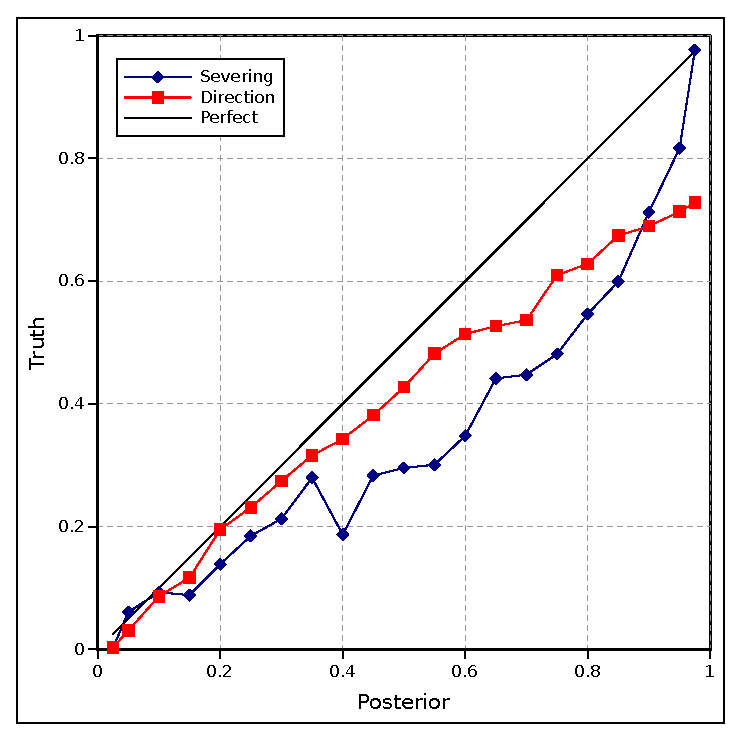
\includegraphics[width=.47\textwidth]{calib}
  \caption{Calibration for the two tests}
\end{figure}

\begin{figure*}[t]
  \begin{tabularx}{\textwidth}{lrllrrr}
Bacterium Of Interest & Level & Helper & Trio-Maker & Sever & PV(trio) & BF(Dir)\\
\hhline{=======}
Bacteroides xylanolyticus & $\leq$3.18E-04 & C. xylanolyticum & D.
formicigenerans &  435.4 & 6.7E-4 & 8.2 \\
\cline{3-6}
& & C. celerecrescens & P. polymyxa &  311.9 & 4.9E-3 &  \\
\cline{3-6}
& & D. formicigenerans & S. termitidis &  173.7 & 1.5E-4 &  \\
\cline{3-6}
& & D. formicigenerans & P. capillosus &  173.7 & 7.4E-3 &  \\
\cline{1-7}
Clostridium methylpentosum & $\leq$9.09E-04 &C. minuta & C. hongkongensis &  431.5 & 4.1E-3 & 110 \\
\cline{1-7}
Coprococcus catus & $\leq$9.02E-04 & P. cinnamivorans & B. cellulosolvens &  117422.9 & 1.4E-3 & 3.4 \\
\cline{3-6}
&  & P. niger & O. valericigenes &  335.3 & 1.8E-3 &  \\
\cline{1-7}
Fusicatenibacter saccharivorans & $\leq$1.34E-03 & R. albus & E. oxidoreducens &  3563.6 & 2.8E-3 & 23 \\
\cline{3-6}
& & C. xylanolyticum & B. viscericola &  2368.6 & 2.3E-3 &  \\
\cline{3-6}
& & D. longicatena & B. dorei &  233.9 & 7.0E-3 &  \\
\cline{1-7}
Ruminococcus faecis & $\leq$1.07E-03 & P. capillosus & E. siraeum &  516.6 & 1.4E-3 & 33 \\
\cline{1-7}
  \end{tabularx}
  \caption{Results of the Three Bacterium Technique.  The three
    bacteria are as described in the Methods section and Level and BF(Dir)
    are as from the previous table.  Sever is the bayes factor
    indicating that the bacterium of interest severs the helper
    bacterium from the disease.  PV(trio) is the highest of the
    p-values by which the trio was established (that is, all six
    p-values are $\leq$ this value).}
\end{figure*}

The three bacterium technique found 3 of the same species as the
gene/bacterium, plus 2 with direction scores between 1 and 10
(i.e. suggestive of causality, but too weak to report on the previous
table).  These species were shown via 1 to 4 helper species each.
This technique also found 21 species whose Gene/ Bacterium direction
scores were less than 1.  Since the direction test is highly reliable
in that range, those are not shown.  The 5 confirmed species are shown
in figure 6.


\subsection{Validation}

Calibration of the direction and severing tests are shown in figure
5.  Both techniques are systematically overconfident, but they stay
fairly close to the
correctly-calibrated line.  While the direction test does better
overall, it is least reliable precisely where we need it most.  The
severing test is less reliable overall, but is robust about when
returning values as strong as are reported here.

\section{Discussion}

\subsection{The Techniques}

The three techniques shown here each have their strengths and
weaknesses.  Applying them together is stronger than any single one.

The Intermediation Technique requires that the gene's effect be
bacterially mediated, and with that requirement not met, it found
nothing.  To put it more positively, the test finds not just one
causal link but two, and its failure to find anything here is itself
interesting.

The Gene/Bacterium Technique requires genomic information, which is
somewhat more difficult to get than microbiome
information.  Also, it relies on the test with the worse calibration.
On the other hand, it has the benefit of simplicity and can find any
relevant bacterium.

The Three Bacterium Technique is worryingly complex and risks errors
because of unconsidered cases.  Also, it can only find bacteria that
are part of trios.  On the other hand, it can be applied to any
disease.

\subsection{Calibration}

The consistent biases of the Direction and Severing tests are
especially worrying.  The reason for this is not clear.  It may be
that dividing PDFs is not similar enough to dividing probabilities.
The difference would be largest with $\chi^2$ scores close to 0, where
the distribution's PDF is steepest, and this would explain why the
direction test fails where it does, though an attempt to smooth the
direction test like the severing test did not improve calibration.
Alternatively, it may also be that the $\chi^2$ distribution is not a
good enough approximation to the actual likelihood of $\chi^2$ scores
when samples are small.  This could be solved by larger data sizes.

In any case, larger data sizes would be valuable.  The indirect
causality patterns that underly these techniques are subtle, and more
data would allow much greater confidence of having found them.

\subsection{The Bacteria}

Eubacterium rectale has
already been associated with ulcerative colitis with hints of a
chemical mechanism\cite{erect}, so finding it here is not terribly
surprising.  

Lactobacillus acidophilus is somewhat more surprising.  It is widely
used as a probiotic, so its causal role is not surprising, but here it
is \textit{high} concentrations of the species that are associated
with disease.  It is possible that modeling microbiomes as ``healthy''
or ``unhealthy'' is too simplistic.  Treatment with Lactobacillus
(albeit rhamnosus, not acidophilus) was nonsignificantly
\textit{harmful} in the two largest studies that tried
it\cite{lgg1,lgg2}.  Alternatively, treating bacterial presences as
scalars may be too simplistic.  L. acidophilus is usually found in the
\textit{jejunum}\cite{lacid}, but these samples are from
\textit{ileum} biopsies.  Perhaps the cause of Crohn's Disease is not
which bacteria are in the intestine, but where in the intestine they
are.

Sphingopyxis alaskensis and Roseiflexus castenholzii are extremely surprising, being marine
bacteria that are not known to colonize intestines at all.  It seems
likely that some other species is being mis-identified -- possibly a
related species, or possibly a species that contaminated the reference
panel that formed NCBI's 16S database.  This casts some doubt on all
other findings, but it seems likely that the well-studied species, at
least, have more robust data.

\subsection{Causal Graph Assumptions}

Throughout this, I have made two simplifying assumptions.  The first
is that the causal graph is simply connected.  This is not likely to
be entirely true, but for any given set of nodes, the simply connected
explanation is the most parsimonious.  This may seem strange from a
machine learning perspective, in which the most general graph is the
fully connected one, but from a biological perspective, each arrow is
a chemical cascade and the simplest explanation contains the fewest.
Also, long-causal-chains are less likely to produce strong evidence
that can be detected from small samples.  Even so, there is one cyclic
motif of particular concern: if three bacteria influence each other in
a circle, and one is influenced by Crohn's Disease, this will pass the
Three Bacterium test.  This may explain the bacteria that passed that
test while emphatically failing the Gene/Bacterium test.

Also, I have assumed there are no interesting selection effects.  If
there were a bacterium that influenced behavior to make healthy people
more likely to volunteer for control groups of observational studies,
both the Gene/Bacterium and Three Bacterium tests would find that it
prevented Crohn's Disease.  There is no way to rule this out from the
data (it would be extremely hard to study!) but it is biologically
implausible.

\subsection{Going Forward}

I am not entirely confident of any of the bacteria listed here.
Nevertheless, they are better starting points for intervention studies
than selecting from the list of correlating species at random.

The observation that NOD2's mechanism of action is probably not
bacterial helps direct investigation of what it might be.  Also, the
observations about displaced L. Acidophilus suggest a new avenue of
investigation.

It is too early to call these techniques validated.  That word should
be reserved for if the bacteria named here prove effective in RCTs.
Nevertheless, I have demonstrated that they can be used on real-world
data, and that the results are plausible.  They may apply to other
diseases.

All code is available on https://github.com/dspeyer/causality/

\begin{thebibliography}{11}
\bibitem{obesity} Tilg \& Kaser ``Gut microbiome, obesity, and metabolic
  dysfunction'' Journal of Clinical Investigation. 2011
\bibitem{autoim} Fung, Garrett, Shahane \& Kwan ``Do Bugs Control Our
  Fate? The Influence of the Microbiome on Autoimmunity'' Curr Allergy
  Asthma Rep. 2012
\bibitem{cns} Wang \& Casper ``The role of microbiome in central
  nervous system disorders'' Brain, Behavior, and Immunity. 2014
\bibitem{rctob} Kadooka et. al. ``Effect of Lactobacillus gasseri SBT2055
  in fermented milk on abdominal adiposity in adults in a randomised
  controlled trial.'' British Journal of Nutrition, 110, pp
  1696-1703. 2013
\bibitem{rctma} Prantera, C. ``Probiotics for Crohn’s Disease: What
  Have We Learned?'' Gut 55.6 (2006): 757–759. PMC. Web. 15 Feb. 2016.
\bibitem{mort} Loftus ``Crohn’s disease: why the disparity in
  mortality?'' Gut 2006
\bibitem{qol}  Gregor et al. ``An evaluation of utility measurement in Crohn's disease'' Inflamm Bowel Dis. 1997
\bibitem{bayesball} Pan \& Xu ``Introduction to Probabilistic
  Graphical Models'' Zhejiang University. 2006
\bibitem{causal} Pearl, J. ``Causal Inference in Statistics: An
  Overview'' Statistical Surveys Vol 3 96-146. 2009
\bibitem{data} Li, Frank \& Sartor, ``Effect of Crohn’s Disease Risk
  Alleles on Enteric Microbiota'' Encyclopedia of Metagenomics. 2014
\bibitem{erect} Joan Vermeiren, Pieter Van den Abbeele, Debby Laukens,
  Louise Kristine Vigsnæs, Martine De Vos, Nico Boon \& Tom Van de
  Wiele ``Decreased colonization of fecal Clostridium
  coccoides/Eubacterium rectale species from ulcerative colitis
  patients in an in vitro dynamic gut model with mucin environment'' FEMS Microbiology Ecology Mar 2012
\bibitem{lgg1} Prantera C, Scribano M L, Falasco G. et al ``Ineffectiveness of probiotics in preventing recurrenece after curative resection for Crohn's disease: a randomised controlled trial with Lactobacillus GG.'' Gut 200251405–409.409
\bibitem{lgg2} Bousvaros A, Guendalini S, Baldassano R N. et al ``A randomized, double blind trial of Lactobacillus GG versus placebo in addition to standard maintenance therapy for children with Crohn's disease.'' Inflamm Bowel Dis 200511833–839.839
\bibitem{lacid} Jens Walter ``Ecological Role of Lactobacilli in the
  Gastrointestinal Tract: Implications for Fundamental and Biomedical
  Research'' Appl. Environ. Microbiol. August 2008

    

\end{thebibliography}


\end{document}
